\documentclass[aspectratio=169]{beamer}

\usepackage{tikz}
\usetikzlibrary{arrows, positioning}
\usepackage{listings}
\usepackage[utf8,latin1]{inputenc}
\usepackage[style = apa, backend = biber, natbib = true]{biblatex}
\addbibresource{../../literature/lit.bib}

\makeatletter \def\newblock{\beamer@newblock} \makeatother  

\beamertemplatenavigationsymbolsempty
\setbeamertemplate{itemize items}[circle]
\setbeamertemplate{section in toc}[circle]
%\mode<beamer>{\setbeamercolor{math text displayed}{fg=iwmorange!50!black}}
\setbeamercolor{block body}{bg=iwmorange!50!white}
\setbeamercolor{block title}{fg=white, bg=iwmorange}

% Definitions for biblatex
\setbeamercolor{bibliography entry note}{fg=iwmgray}
\setbeamercolor{bibliography entry author}{fg=iwmgray}
\setbeamertemplate{bibliography item}{}

\definecolor{iwmorange}{RGB}{255,105,0}
\definecolor{iwmgray}{RGB}{67,79,79}
\setbeamercolor{title}{fg=iwmorange}
\setbeamercolor{frametitle}{fg=iwmorange}
\setbeamercolor{structure}{fg=iwmorange}
\setbeamercolor{normal text}{fg=iwmgray}
\setbeamercolor{author}{fg=iwmgray}
\setbeamercolor{date}{fg=iwmgray}
%\color{white}

\newcommand{\vect}[1]{\mathbf{#1}}
\newcommand{\mat}[1]{\mathbf{#1}}
\newcommand{\gvect}[1]{\boldsymbol{#1}}
\newcommand{\gmat}[1]{\boldsymbol{#1}}

\lstset{language=R,%
  %backgroundcolor=\color{iwmgray!80!white},
  basicstyle=\ttfamily\color{iwmorange},
  frame=single,
  commentstyle=\slshape\color{black},
  keywordstyle=\bfseries\color{white},
  identifierstyle=\color{white},
  stringstyle=\color{green!85!black},
  numbers=none,%numberstyle=\tiny,
  basewidth={.5em, .4em},
  showstringspaces=false,
  emphstyle=\color{red!50!white}}

\lstdefinestyle{plain}{language=R,
  frame=none,
  basicstyle=\ttfamily\color{iwmorange},
  commentstyle=\slshape\color{iwmgray},
  keywordstyle=\bfseries\color{iwmgray},
  identifierstyle=\color{iwmgray},
  stringstyle=\color{iwmgray},
  numbers=none,
  basewidth={.5em, .4em},
  showstringspaces=false}

\AtBeginSection[]{
  \frame{
    \tableofcontents[sectionstyle=show/hide, subsectionstyle=show/show/hide]}}

\setbeamertemplate{headline}{
 \begin{beamercolorbox}{section in head}
   \vskip5pt\insertsectionnavigationhorizontal{\paperwidth}{}{}\vskip2pt
 \end{beamercolorbox}
}

\setbeamertemplate{footline}{\vskip-2pt\hfill\insertframenumber$\;$\vskip2pt}

\title{Power simulation for linear mixed-effects models}
\author{Nora Wickelmaier}
\date{February 6, 2023}

\begin{document}

\begin{frame}
\thispagestyle{empty}
\titlepage
\end{frame}

% \begin{frame}{Outline}
% \tableofcontents
% \end{frame}

% \section{Simple regression}
% 
% \begin{frame}{Example: \citet{Fox2008}}
%   \begin{itemize}
%     \item Vocabulary Data from the U.S.\ General Social Surveys
%     \item $N = \text{21,638}$
%     \item Outcome:
%       \begin{itemize}
%         \item Vocabulary score
%       \end{itemize}
%     \item Predictor:
%       \begin{itemize}
%         \item Years of education
%       \end{itemize}
%   \end{itemize}
% \end{frame}
% 
% \begin{frame}{Example: \citet{Fox2008}}
% \begin{columns}
%   \column{.6\textwidth}
%   \includegraphics[scale=.8]{../figures/voc}
%   \column{.4\textwidth}
%   \begin{align*}
%     y_{i} & = \beta_0 + \beta_1 x_{i} + \varepsilon_i\\
%     \varepsilon_i & \sim N(0, \sigma^2)
%   \end{align*}
%   \begin{tabular}{lr}
%     \hline
%          &  Mean (SD) \\
%     \hline
%     Vocabulary &  6.00 (2.17)\\
%     Education  & 12.80 (3.04)\\
%     \hline
%   \end{tabular}
% \end{columns}
% \end{frame}
% 
% \begin{frame}{}
%   \begin{block}{Exercise}
%     \begin{itemize} 
%       \item What are good assumptions about the distributions of
%         \begin{itemize}
%           \item Vocabulary
%           \item Education
%         \end{itemize}
%     \end{itemize}
%   \end{block}
% \end{frame}
% 
% {\setbeamercolor{background canvas}{bg=iwmgray!80!white}
% 
% \begin{frame}[fragile]{Vocabulary data}
%   \begin{lstlisting}
% dat <- read.table("Vocabulary.txt", header=TRUE, 
%                   stringsAsFactors=TRUE)
% 
% lm1 <- lm(vocabulary ~ education, dat)
% summary(lm1)
% 
% plot(jitter(vocabulary, 2) ~ jitter(education, 2),
%      dat, pch=".", xlab="Years of education",
%      ylab="Vocabulary score", col="darkgrey")
% abline(lm1)
%   \end{lstlisting}
% \end{frame}
% 
% }

\begin{frame}{Power analysis by simulation}
  Why simulation?
  \begin{itemize}
    \item Simulation is at the heart of statistical inference
    \item Inference: Compare the data with the output of a statistical model
    \item If data look different from model output, reject model (or its assumptions)
    \item Simulation forces us to {\bf specify a data model} and to attach
      meaning to its components
    \item Model should not be totally unrealistic for those aspects of the
      world we want to learn about
  \end{itemize}
  \nocite{Wickelmaier2022}
\end{frame}

\begin{frame}{Specify the model including the effect of interest}
(1) Choose statistical model according to its assumptions
  \begin{itemize}
    \item Binomial test $\to$ binomial distribution $\to$ \texttt{rbinom()}
    \item t test $\to$ normal distribution $\to$ \texttt{rnorm()}
    \item \dots
  \end{itemize}
(2) Fix unknown quantities
  \begin{itemize}
    \item Standard deviations, correlations, \dots
%    \item Plausible values from the literature (beware of significance filter)
  \end{itemize}
(3) Specify the effect of interest
  \begin{itemize}
    \item Smallest effect size of interest (SESOI)
%    \item Not the true effect (else no need to run the study!)
%    \item Not the effect one expects or hopes to find (size of effect is unknown!)
%    \item Never an effect size taken from another study (significance filter!)
%    \item But the biologically or clinically or psychologically ``relevant
%      effect one would regret missin'' (Harrell, 2020)
  \end{itemize}
\end{frame}

\begin{frame}[fragile]{Estimating power with simulation}
  {Pseudo code}
\begin{lstlisting}[style=plain, frame=single]
Set sample size
replicate
{
  Draw sample from model with minimal relevant effect
  Test null hypothesis
}
Determine proportion of significant results
\end{lstlisting}
Sample size calculation
  \begin{itemize}
    \item Adjust $n$ until desired power (0.8 or 0.95) is reached
    \item To be on the safe side, assume higher variation, less (or more)
      correlation, and smaller interesting effects (what results can we
      expect, if \dots)
  \end{itemize}
\end{frame}

% {\setbeamercolor{background canvas}{bg=iwmgray!80!white}
% 
% \begin{frame}[fragile]{Power simulation}
%   \begin{lstlisting}
% n <- 150
% 
% prob <- table(dat$education) / nrow(dat)
% simdat <- data.frame(x1 = sample(0:20, n, TRUE, prob))
% 
% pval <- replicate(2000, {
%         y <- 1.5 + 0.2*simdat$x1 + rnorm(n, sd=2.2)
%         m1 <- lm(y ~ 1, simdat)
%         m2 <- lm(y ~ x1, simdat)
%         anova(m1, m2)$"Pr(>F)"[2]
% })
% mean(pval < 0.05)
%   \end{lstlisting}
% \end{frame}
% 
% }


\begin{frame}[fragile]{Generalized linear models}
  \begin{itemize}
    \item A generalized linear model is defined by
\[
  g(E(y)) = \beta_0 + \beta_1 x_1 + \beta_2 x_2 + \cdots + \beta_k x_k,
\]
where $g()$ is the link function that links the mean to the linear predictor.
The response $y$ is assumed to be independent and to follow a distribution
from the exponential family

\item In R, a GLM is fitted by

  \begin{lstlisting}[style=plain]
  glm(y ~ x1 + x2 + ... + xk, family(link), data)
\end{lstlisting}
  \end{itemize}
\end{frame}


\begin{frame}{Binomial regression}
  \begin{itemize}
    \item Logit or probit models are special cases of GLMs for binomial
      response variables
    \item Artificial example: congenital eye disease
  \end{itemize}
\begin{columns}[c]
\begin{column}{6cm}
  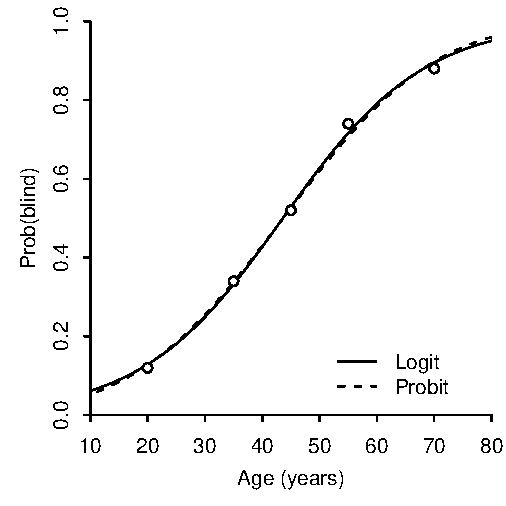
\includegraphics[scale=.7]{../figures/glm}
\end{column}
\begin{column}{5cm}
Logit model
\[
  \log\frac{p}{1 - p} = \beta_0 + \beta_1 AGE
\]
Probit model
\[
  \Phi^{-1}(p) = \beta_0 + \beta_1 AGE
\]
\end{column}
\end{columns}
\end{frame}

\begin{frame}{Logit model / logistic regression}
  \begin{itemize}
    \item We want to model the probability of $y$ with the logistic
      function
  \begin{equation*}
    p(y) = \frac{1}{1 + e^{-y}}~~\text{  with } y \sim Binom(n, p)
  \end{equation*}
    \item How do we get the logit model $\log\frac{p}{1 - p} =
      \beta_0 + \beta_1 x$ from that?
  \end{itemize}
      \begin{align*}
        \log\left(\frac{p}{1 - p}\right) = \log(p) - \log(1-p) 
        & = \log\left(\frac{1}{1 + e^{-y}}\right) - \log\left(1 - \frac{1}{1 + e^{-y}}\right) \\
        & = \log(1) - \log(1 + e^{-y}) - \log(e^{-y}) + \log(1 + e^{-y}) \\
        & = -\log(e^{-y})\\
        & = y := \beta_0 + \beta_1 x
      \end{align*}
     with \color{iwmorange}{$1 - \frac{1}{1 + e^{-y}} = \frac{e^{-y}}{1 + e^{-y}}$}
\end{frame}

\begin{frame}{Refresher: Logarithm rules}

\begin{tabular}{p{2cm}l}
  Product:  & $\log(xy)=\log x+\log y$ \\
  &\\
  Quotient: & $\log\!{\frac {x}{y}}=\log x-\log y$ \\
  &\\
  Power:    & $\log\left(x^{p}\right)=p\log x$ \\
  &\\
  Root:     & $\log{\sqrt[{p}]{x}}={\frac {\log x}{p}}$ \\
\end{tabular}

\end{frame}

\begin{frame}{Meta-information and Memory: Nicole's experiment}
      \begin{columns}
        \begin{column}[c]{.62\textwidth}
    {\color{iwmorange}Task:}\\
          Participants read 40 sentences that can be either true (30)
      or false (10) which are presented in different font colors\\ 
        \end{column}
        \begin{column}[c]{.3\textwidth}
      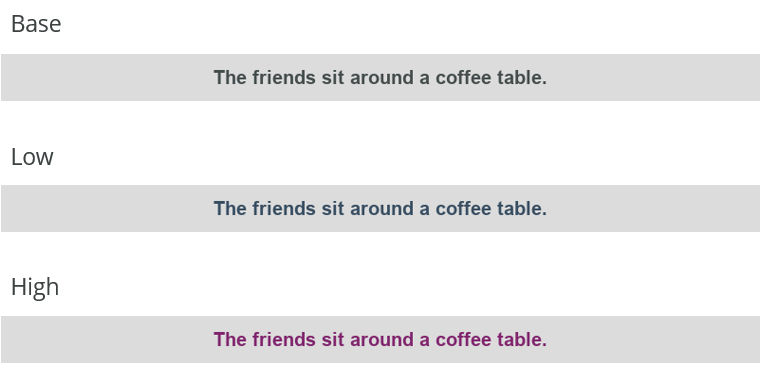
\includegraphics[scale = .3]{../figures/material}
        \end{column}
      \end{columns}

  {\color{iwmorange}Study 1:}\\
  Recognition Memory: ``Did you read this statement?''\\
      DV -- correct answer: correct recall\\
      IVs -- condition (control vs.\ high vs.\ low discriminability)\\
      ~~~~~-- truthvalue (true vs.\ false)

    {\color{iwmorange}Study 2:}\\
    Source Memory: ``Was this statement true, false, or
      new?''\\
      DV -- correct answer: true sentence classified as true\\
      IVs -- condition (high vs.\ low discriminability)\\
      ~~~~~-- truthvalue (true vs.\ false)
\end{frame}

\begin{frame}{Meta-information and Memory: Nicole's experiment}
  {Hypotheses}
  \begin{itemize}
    \item[Study 1] Recognition Memory:\\
      Significant interaction effect between truthvalue and
      discriminability: Recognition memory will be higher for true than
      false statements when a discriminability task is present
    \item[Study 2] Source Memory:\\
      Significant interaction effect between truthvalue and
      discriminability: Participants in high discriminability condition
      will more often classify statements correctly as true or false than
      in the low discriminability condition
  \end{itemize}
  \vspace{.5cm}
  \pause
  $\to$ We have the data of the first study and want to calculate the
  {\bf number of participants} we need for the second study
\end{frame}


\begin{frame}[fragile]{Meta-information and Memory: Nicole's experiment}
  {Model}
  \begin{itemize}
    \item In order to test the interaction, we fit the following model:
  \begin{equation*}
    log\left(\frac{P(correct)}{P(false)}\right) = \beta_0 + \beta_1 truthval + \beta_2 cond +
    \beta_3 (truthval \times cond) + \upsilon_0 + \eta_0
  \end{equation*}
  with $\upsilon_0 \sim N(0, \sigma_{\upsilon})$ and $\eta_0 \sim N(0,
  \sigma_{\eta})$, all random effects i.i.d.
\item This model can be fitted in R with
  \begin{lstlisting}[style = plain, frame = single]
lme4::glmer(correctAnswer ~ truthvalue * condition + 
            (1|participantID) + (1|itemID),
            data, family = binomial)
\end{lstlisting}
  \end{itemize}

  \pause
  $\to$ How many parameters does this model have?
\end{frame}


\begin{frame}{Estimates from Study 1}
\begin{tabular}{lrr}
  \hline
  {\bf Random effects} & Variance & Std.Dev. \\ 
  \hline
itemID          & 0.29 & 0.54 \\ 
participantID   & 0.58 & 0.76 \\ 
   \hline
\end{tabular}

\vspace{.5cm}

\begin{tabular}{lrrrr}
  \hline
  {\bf Fixed effects} & Estimate & Std. Error & z value & Pr($>$$|$z$|$) \\ 
  \hline
  (Intercept)                   &  1.62 & 0.15 & 11.15 & 0.00 \\ 
  truthvaluetrue                & -0.02 & 0.12 & -0.16 & 0.87 \\ 
  conditionhigh                 & -0.50 & 0.19 & -2.59 & 0.01 \\ 
  conditionlow                  & -0.64 & 0.19 & -3.35 & 0.00 \\ 
  truthvaluetrue:conditionhigh  &  0.39 & 0.16 &  2.44 & 0.01 \\ 
  truthvaluetrue:conditionlow   &  0.40 & 0.16 &  2.48 & 0.01 \\ 
   \hline
\end{tabular}

\vspace{.5cm}
\pause
$\to$ Parameters are on the logit scale
\end{frame}

\begin{frame}{Model predictions}
\centering
\begin{tabular}{ccrl}
  \hline
 truthvalue & condition & prob & logit \\ 
  \hline
% false & control & 0.79 & obs \\ 
% true & control & 0.80 & obs \\ 
% false & high & 0.72 & obs \\ 
% true & high & 0.78 & obs \\ 
% false & low & 0.70 & obs \\ 
% true & low & 0.76 & obs \\ 
 false & control & 0.84 & 1.62  \\ 
 true  & control & 0.83 & 1.60  \\ 
 false & high    & 0.76 & 1.13  \\ 
 true  & high    & 0.82 & 1.50  \\ 
 false & low     & 0.73 & 0.98  \\ 
 true  & low     & 0.80 & 1.36  \\ 
 \hline
% false & control & 1.62 & logit \\ 
% true  & control & 1.60 & logit \\ 
% false & high    & 1.13 & logit \\ 
% true  & high    & 1.50 & logit \\ 
% false & low     & 0.98 & logit \\ 
% true  & low     & 1.36 & logit \\ 
%   \hline
\end{tabular}
\end{frame}

\begin{frame}[fragile]{Predictions on the logit scale}
  \begin{columns}
    \begin{column}[c]{.3\textwidth}
      {\small
      \begin{tabular}{@{}lr@{}}
        \hline
        & est \\
        \hline
       (Intercept)           &  1.62 \\
       truthvaltrue          & -0.02 \\
       condhigh              & -0.50 \\
       condlow               & -0.64 \\
       truthvaltrue:condhigh &  0.39 \\
       truthvaltrue:condlow  &  0.40 \\
        \hline
       \end{tabular}
       }

       \vspace{.3cm}
Get predictions:
\begin{lstlisting}[style = plain]
  predict(glm1,
          re.form = NA)
\end{lstlisting}
    \end{column}
    \begin{column}[c]{.7\textwidth}
      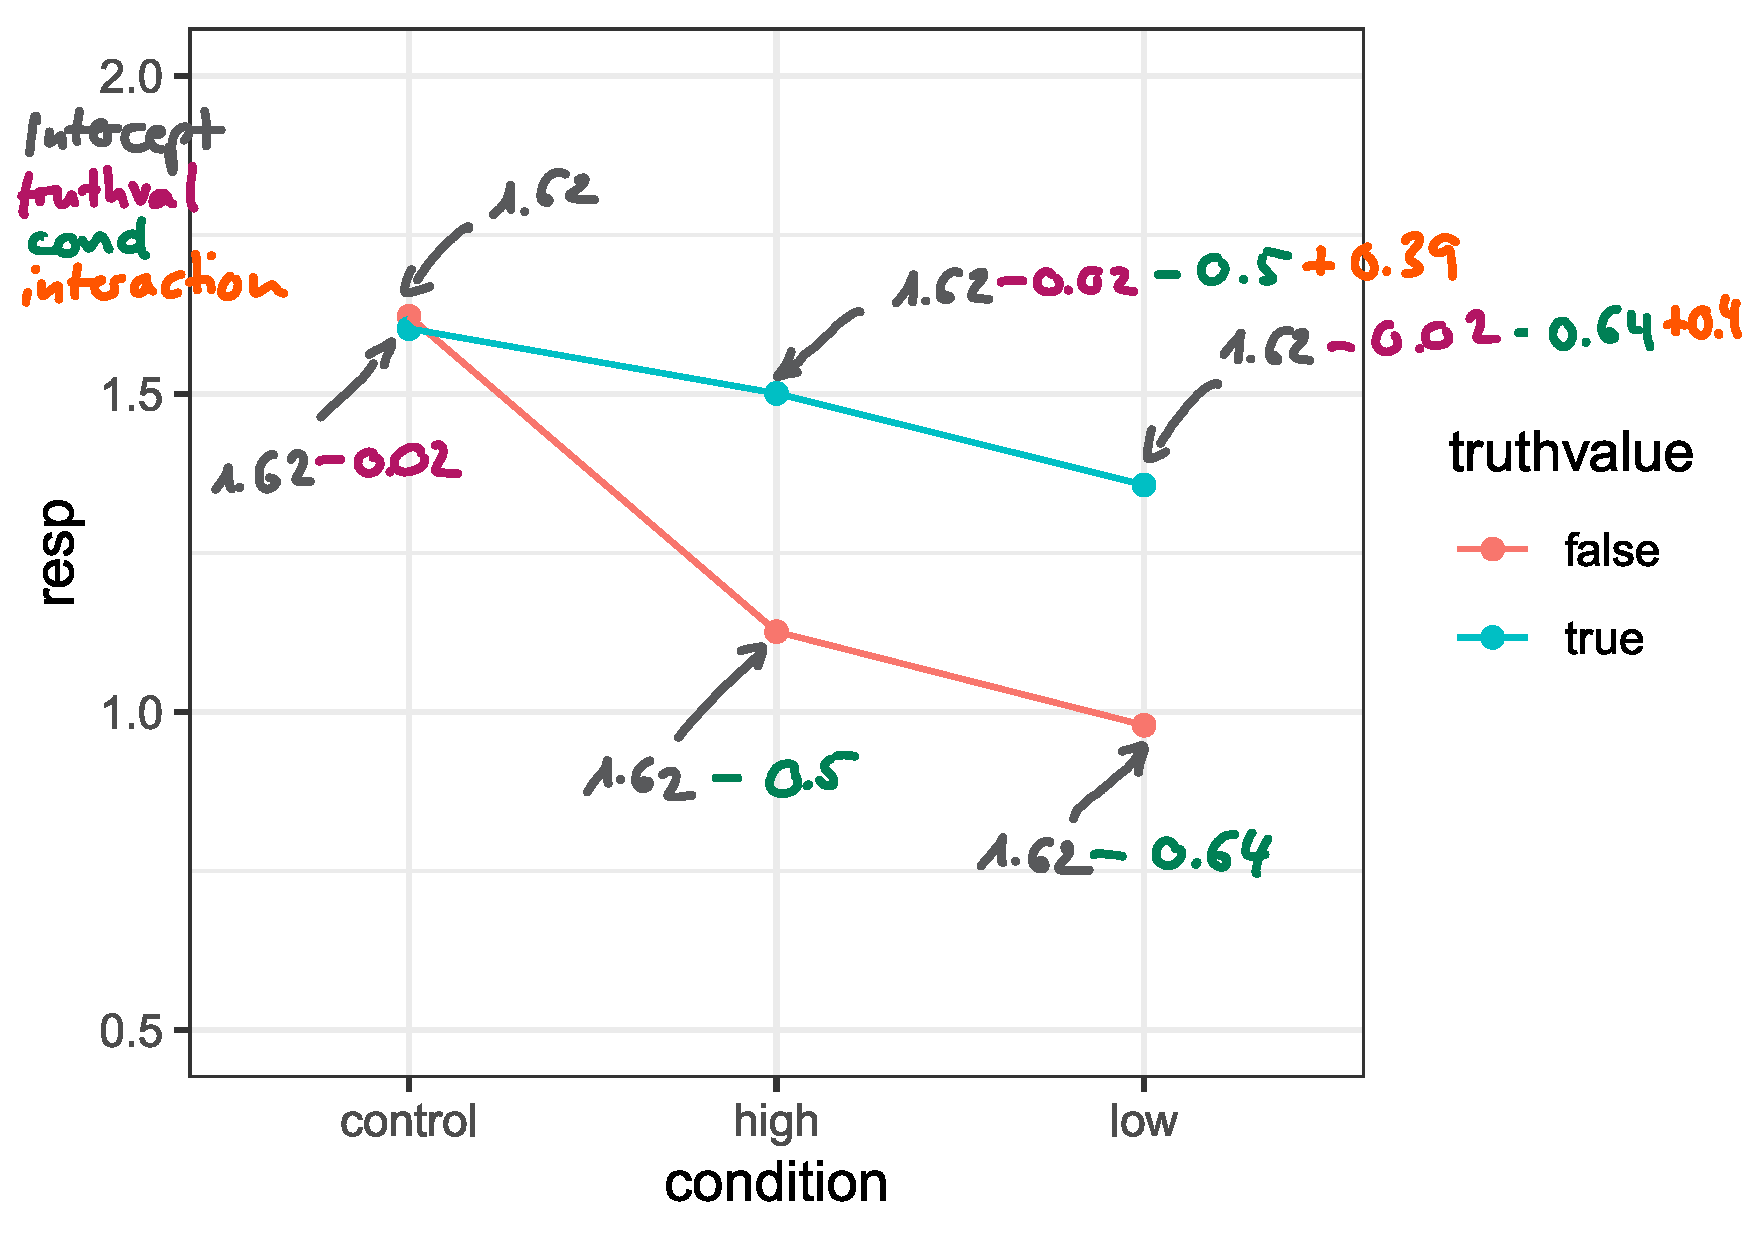
\includegraphics[scale = .35]{../figures/predlogit_with_params}
    \end{column}
  \end{columns}
\end{frame}

\begin{frame}[fragile]{Predictions on the probability scale}
  \begin{columns}
    \begin{column}[c]{.3\textwidth}
      {\small
      \begin{tabular}{@{}lr@{}}
      \hline
 & OR \\ 
  \hline
  (Intercept) & 5.06 \\ 
  truthvaltrue & 0.98 \\ 
  condhigh & 0.61 \\ 
  condlow & 0.53 \\ 
  truthvaltrue:condhigh & 1.48 \\ 
  truthvaltrue:condlow & 1.49 \\ 
   \hline
\end{tabular}
      }

\vspace{.3cm}
Get predictions:
\begin{lstlisting}[style = plain]
  predict(glm1, 
          re.form = NA,
          type = "resp")
\end{lstlisting}
    \end{column}
    \begin{column}[c]{.7\textwidth}
      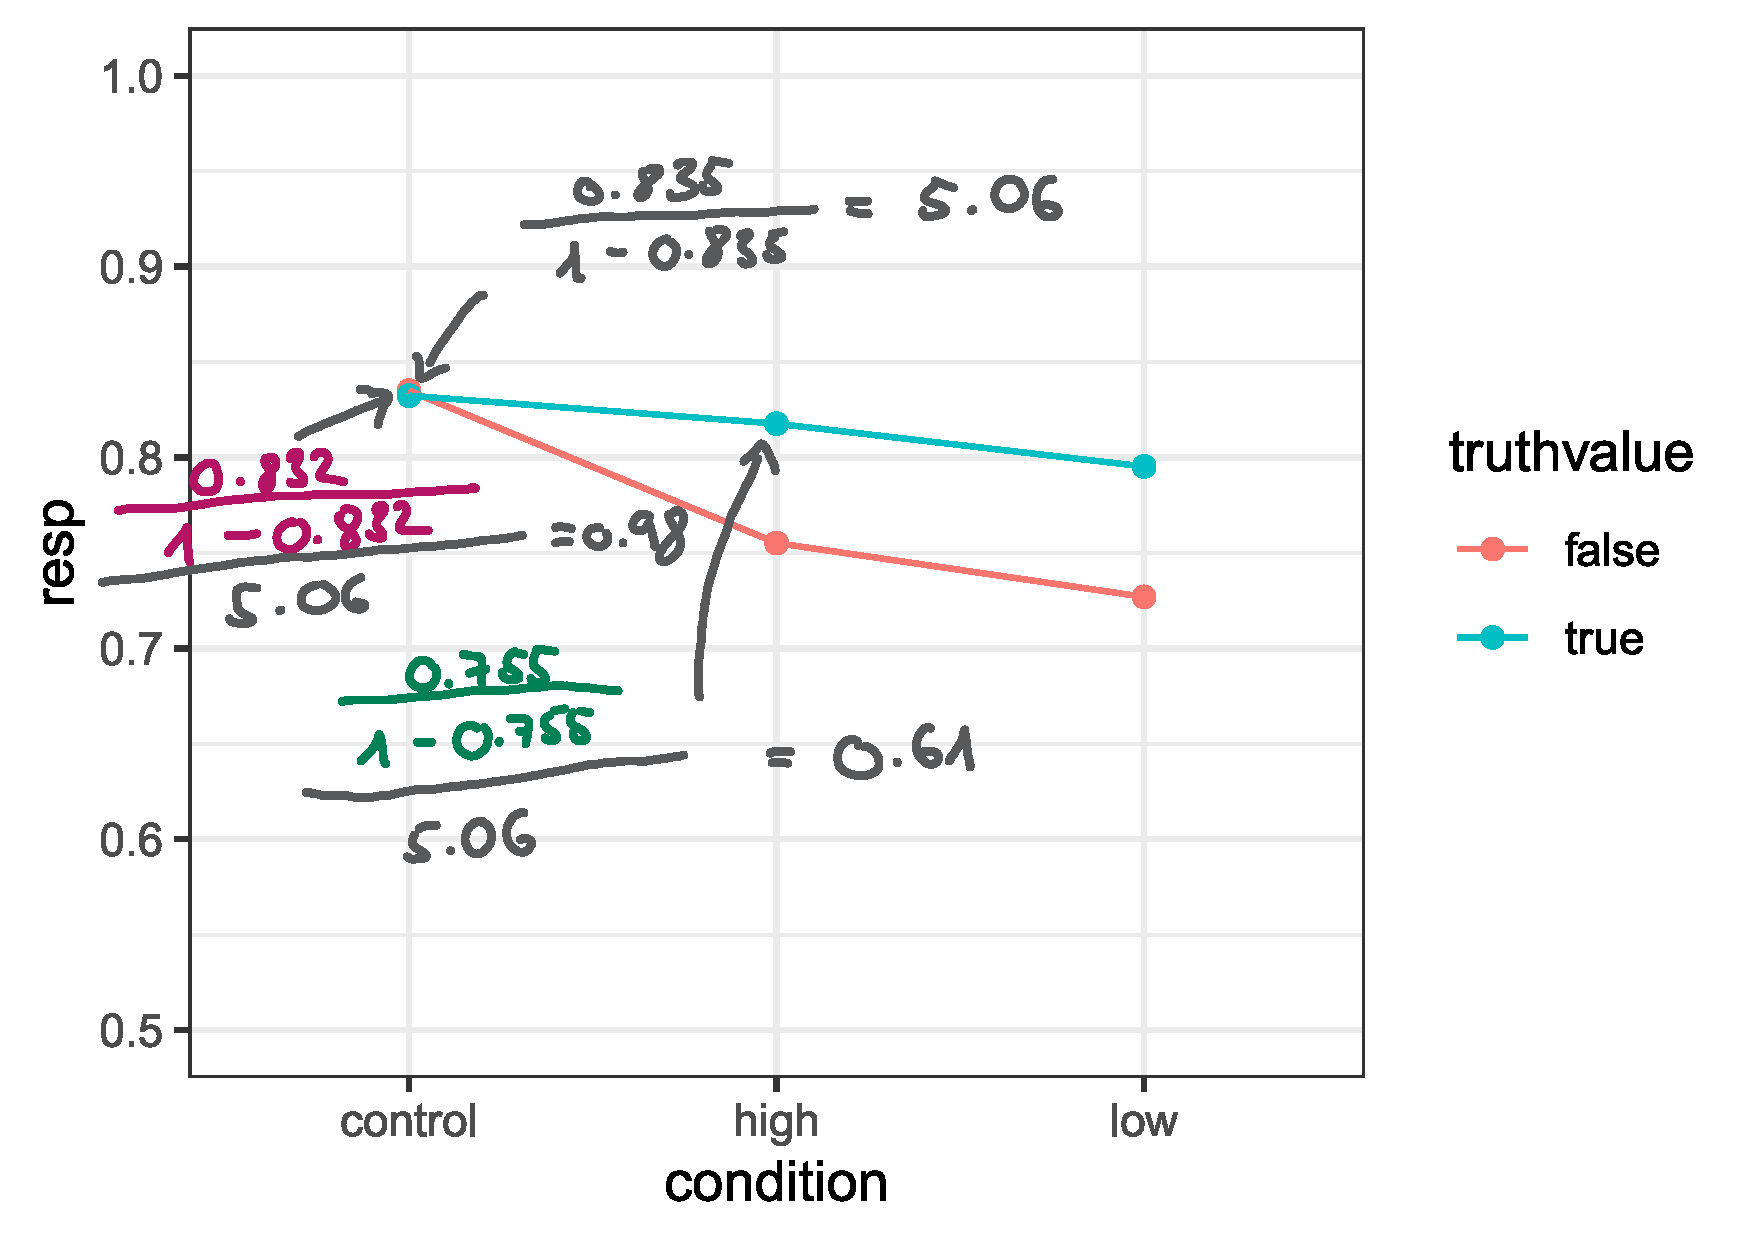
\includegraphics[scale = .35]{../figures/predprob_with_params}
    \end{column}
  \end{columns}
\end{frame}

{\setbeamercolor{background canvas}{bg=iwmgray!80!white}

\begin{frame}[fragile]{Data simulation for Study 2}
\begin{lstlisting}
n <- 200    # try different values

# Create data frame
dat <- data.frame(
    id         = factor(rep(1:n, each = 40)),
    item       = factor(paste(rep(1:5, each = 40), 1:40, sep = ":")),
    condition  = factor(rep(c("high", "low"), each = nitem)),
    truthvalue = factor(rep(c("true", "false"), c(30, 10)))
)

# Do some checks
xtabs( ~ id + item, dat)
xtabs( ~ condition + truthvalue, dat)
xtabs( ~ condition + truthvalue + id, dat)
\end{lstlisting}
\end{frame}

}


\begin{frame}{Effect size of interest}
  How do I find suitable numbers for the model parameters?

  Let us simulate some data with minimal error and plot the results.
\begin{columns}
  \begin{column}[c]{.7\textwidth}
    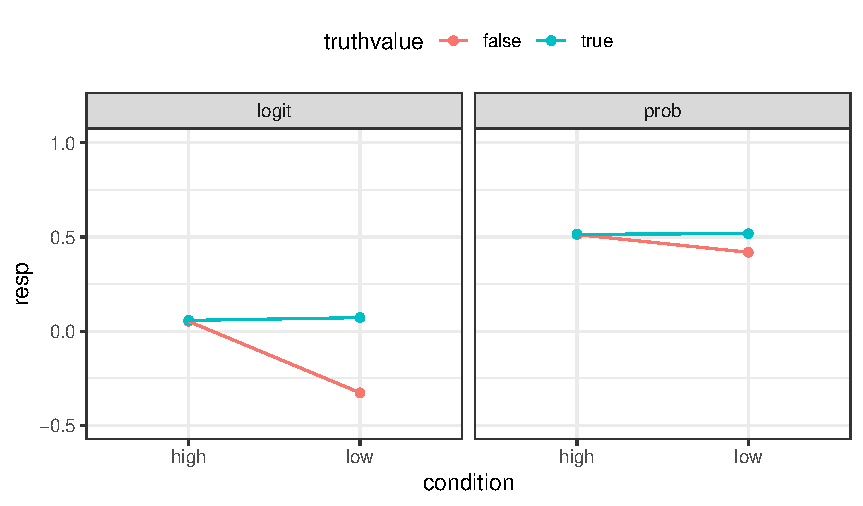
\includegraphics[scale = .7]{../figures/find_params}
  \end{column}
  \begin{column}[c]{.3\textwidth}
    {\footnotesize
        \begin{tabular}{@{}lrrrr}
  \hline
 & ``true'' \\ 
  \hline
  (Intercept)          &  0.00 \\ 
  truthvaltrue         &  0.05 \\ 
  condlow              & -0.40  \\ 
  truthvaltrue:condlow &  0.40 \\ 
   \hline
\end{tabular}
%
%    \begin{tabular}{@{}lrrrr}
%  \hline
% & Est. \\ 
%  \hline
%  (Intercept)          &  0.04 \\ 
%  truthvaltrue         &  0.02 \\ 
%  condlow              & -0.36  \\ 
%  truthvaltrue:condlow &  0.38 \\ 
%   \hline
%\end{tabular}
    }
  \end{column}
\end{columns}

\end{frame}

{\setbeamercolor{background canvas}{bg=iwmgray!80!white}


\begin{frame}[fragile]{Data simulation for Study 2}
\begin{lstlisting}
ran <- c("id.(Intercept)"   = 0.6,
         "item.(Intercept)" = 0.8)
fix <- c("(Intercept)"                 = 0, 
         "truthvaluetrue"              = 0.05,
         "conditionlow"                = -0.4,
         "truthvaluetrue:conditionlow" = 0.4)

# Simulate data
sim <- simulate( ~ truthvalue * condition + (1|id) + (1|item),
                newdata   = dat,
                newparams = list(beta = fix, theta = ran),
                family    = binomial,
                nsim      = 20) # should be at least 400!
\end{lstlisting}
\end{frame}


\begin{frame}[fragile]{Power simulation}
\begin{lstlisting}
pval <- numeric(ncol(sim))

for (i in seq_len(ncol(sim))) {
  m1 <- glmer(sim[, i] ~ truthvalue * condition + 
                (1|id) + (1|item), dat, family = binomial)
  pval[i] <- summary(m1)$coef["truthvaluetrue:conditionlow", "Pr(>|z|)"]
}

# Power
mean(pval < 0.05)
hist(pval)
\end{lstlisting}
\end{frame}

\begin{frame}[fragile]{Parameter recovery}
\begin{lstlisting}
par_rev <- replicate(400, {
  sim <- simulate( ~ truthvalue*condition + (1|id) + (1|item),
                  newdata = dat,
                  newparams = list(beta = c(0, 0.01, -0.2, 0.2),
                                   theta = c(0.5, 0.5)),
                  family = binomial)[,1]
  glmer(sim ~ truthvalue * condition + (1|id) + (1|item), 
        data = dat, family = binomial)
  })
mean(sapply(par_rev, fixef)[1,]); mean(sapply(par_rev, fixef)[2,])
mean(sapply(par_rev, fixef)[3,]); mean(sapply(par_rev, fixef)[4,])

mean(sqrt(sapply(par_rev, function(x) unlist(VarCorr(x)))[1,]))
mean(sqrt(sapply(par_rev, function(x) unlist(VarCorr(x)))[2,]))
\end{lstlisting}
\end{frame}

}
 
\begin{frame}{Estimation of inflated effect}
  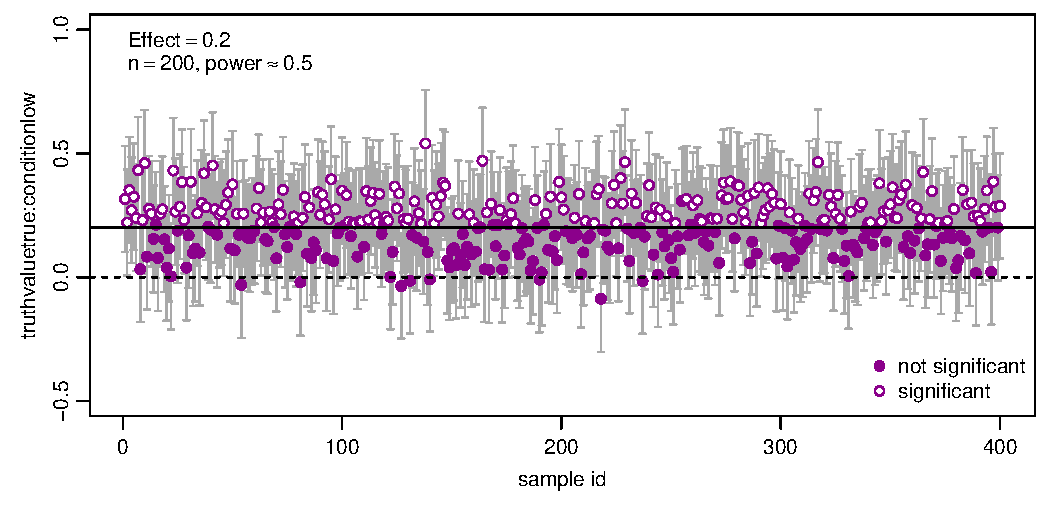
\includegraphics[scale = .8]{../figures/inflation}
\end{frame}

{\setbeamercolor{background canvas}{bg=iwmgray!80!white}

\begin{frame}[fragile]{Estimation of inflated effect}
\begin{lstlisting}
# Parameter estimates and confidence intervals
int <- sapply(par_rev, 
  function(x) fixef(x)["truthvaluetrue:conditionlow"])
ci <- sapply(par_rev, 
  function(x) confint(x, method = "Wald")["truthvaluetrue:conditionlow",])
# p values
p <- sapply(par_rev, 
  function(x) summary(x)$coef["truthvaluetrue:conditionlow", "Pr(>|z|)"])

# Power
mean(p < 0.05)
hist(p)
# Inflation of effect
summary(int[p < 0.05])
\end{lstlisting}
\end{frame}

}

\begin{frame}{Results of Study 2}
  \begin{columns}
    \begin{column}[c]{.5\textwidth}
      {\footnotesize
      \begin{tabular}{@{}lrrrr@{}}
  \hline
 & est & se & z & p \\ 
  \hline
(Intercept) & -0.53 & 0.08 & -6.66 & 0.00 \\ 
  truthvaltrue & 1.34 & 0.07 & 18.72 & 0.00 \\ 
  condlow & -0.21 & 0.11 & -1.90 & 0.06 \\ 
  truthvaltrue:condlow & 0.08 & 0.10 & 0.74 & 0.46 \\ 
   \hline
\end{tabular}
      }
    \end{column}
    \begin{column}[c]{.5\textwidth}
      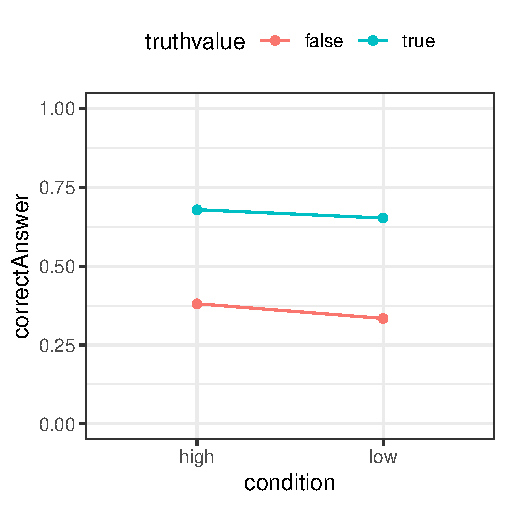
\includegraphics[scale = .8]{../figures/study2}
    \end{column}
  \end{columns}
\end{frame}

% \begin{frame}{Linear mixed-effects models}
% 
% {\small
% \[
%   \begin{pmatrix}
%     y_{11}\\
%     \vdots\\
%     y_{ij}\\
%     \vdots\\
%     y_{qn}
%   \end{pmatrix}
%   =
%   \begin{pmatrix}
%     1 & x_{111} & x_{121} & \dots & x_{1p1}\\
%     1 & x_{112} & x_{122} & \dots & x_{1p2}\\
%     \vdots & \vdots & \vdots && \vdots \\
%     1 & x_{211} & x_{221} & \dots & x_{2p1}\\
%     \vdots & \vdots & \vdots && \vdots \\
%     1 & x_{n1q} & x_{n2q} & \dots & x_{npq}\\
%   \end{pmatrix}
% \times
%   \begin{pmatrix}
%     \beta_0\\
%     \beta_1\\
%     \vdots\\
%     \beta_p
%   \end{pmatrix}
% +
%   \begin{pmatrix}
%     1 & 0 & \dots & 0 & 0\\
%     \vdots & \vdots && \vdots & \vdots \\
%     0 & 1 & \dots & 0 & 0\\
%     \vdots & \vdots && \vdots & \vdots \\
%     0 & 0 & \dots & 1 & 0\\
%     \vdots & \vdots && \vdots & \vdots \\
%     0 & 0 & \dots & 0 & 1
%   \end{pmatrix}
% \times
%   \begin{pmatrix}
%     \upsilon_1\\
%     \vdots\\
%     \upsilon_{qn}\\
%   \end{pmatrix}
% +
%   \begin{pmatrix}
%     e_{11}\\
%     \vdots\\
%     e_{ij}\\
%     \vdots\\
%     e_{qn}
%   \end{pmatrix}
% \]
% }
% and the corresponding vector equation
% \[
%   \mat{y} = \mat{X} \, \gmat{\beta} + \mat{Z} \,\gmat{\upsilon} + \mat{e}
% \]
% \
% \end{frame}
%
% \section{Mixed-effects regression}
% 
% \begin{frame}{Example: \citet{Bauer2005}}
%   \begin{itemize}
%     \item $N = \text{7,185}$
%     \item 160 schools
%     \item Outcome:
%       \begin{itemize}
%         \item math achievement ($\bar y = 12.75, sd = 6.88$)
%       \end{itemize}
%     \item Predictors:
%       \begin{enumerate}
%         \item child SES (metric, group mean centered with $sd = .66$)
%         \item school sector ($0 = \text{public school}$, $1 = \text{private
%           school}$, 49\,\% of schools were private)
%         % \item disciplinary climate (metric, high values reflect greater
%         %   disciplinary problems, grand mean centered with $sd = .94$)
%       \end{enumerate}
%   \end{itemize}
% \end{frame}
% 
% \begin{frame}{Statistical model}
%   \begin{align*}
%     y_{ij} = & \beta_{0} + \beta_{1}cses_{ij} + \beta_{2}meanses_{i} +
%     \beta_{3}sector_{i}\\
%     & + \beta_{4}(cses_{ij} \times meanses_i) +
%     \beta_5(cses_{ij}\times sector_i)\\
%     & + \upsilon_{0i} + \upsilon_{1i}cses_{ij} + \varepsilon_{ij}
%   \end{align*}
%   \[
%     \begin{pmatrix}
%       \upsilon_{0i} \\
%       \upsilon_{1i}
%     \end{pmatrix}
%     \sim N\left(
%     \begin{pmatrix}
%       0 \\
%       0
%     \end{pmatrix},
%     \gmat{\Sigma}_{\upsilon} = 
%     \begin{pmatrix}
%       \sigma_{\upsilon_{0}}^2 & \sigma_{\upsilon_{0}\upsilon_1} \\
%       \sigma_{\upsilon_{0}\upsilon_1} & \sigma_{\upsilon_{1}}^2
%     \end{pmatrix}
%     \right) \text{i.i.d.},~~~\varepsilon_i \sim N(\vect{0}, \sigma^2
%     \mat{I}_{n_i})~\text{i.i.d.}
%   \]
%   \[
%     i = 1,\dots,I, ~~~ j=1,\dots,n_i
%   \]
% 
% \end{frame}
% 
% {\setbeamercolor{background canvas}{bg=iwmgray!80!white}
% 
% \begin{frame}[fragile]{Highschool and beyond data}
%   \begin{lstlisting}
% library(lme4)
% dat <- read.table("hsbdataset.txt", header=TRUE)
% 
% # Look at standard deviations
% sd(dat$ses)
% sd(dat$cses)
% table(dat$sector) / nrow(dat)
% 
% lme1 <- lmer(mathach ~ cses*meanses + cses*sector + 
%             (cses | school), dat)
% summary(lme1)
% 
% library(lattice)
% xyplot(mathach ~ cses | as.factor(sector), dat, 
%        groups=school, type="r")
%   \end{lstlisting}
% \end{frame}
% 
% 
% \begin{frame}[fragile]{Simulate data frame}
%   \begin{lstlisting}
% nschool <- 150
% nstudent <- 40
% simdat <- data.frame( 
%               id = seq_len(nstudent),
%               school = seq_len(nschool),
%               sector = rep(0:1, each=nschool/2),
%               ses = rnorm(nschool*nstudent, 0, .8)
%           )
% 
% # Mean centering ses
% simdat$meanses <- ave(simdat$ses, simdat$school)
% simdat$cses <- simdat$ses - simdat$meanses
%   \end{lstlisting}
% \end{frame}
% 
% \begin{frame}[fragile]{Define parameters}
%   \begin{lstlisting}
% se  <- 6.5
% sp  <- 1.6
% spw <- 0.3
% cov <- 0.4*sp*spw
% 
% fix <- c("(Intercept)"=12, meanses=5, cses=2.5, 
%          sector=1, "cses:meanses"=0.7, 
%          "cses:sector"=-0.7)
% 
% mat <- matrix(c(sp^2, cov,
%                 cov, spw^2), 2, 2)
% ran <- chol(mat) / se
% 
% params <- list(theta=t(ran)[lower.tri(t(ran), TRUE)],
%                beta=fix, sigma=se)
%   \end{lstlisting}
% \end{frame}
% 
% 
% \begin{frame}[fragile]{Power simulation}
%   \begin{lstlisting}
% pval <- replicate(200, {
%   mathach <- simulate(~ cses*meanses + cses*sector + 
%                      (cses | school),
%                      newparams=params, newdata=simdat,
%                      family=gaussian)$sim_1
%   m1 <- lmer(mathach ~ meanses + cses + sector
%              + (cses | school), simdat, REML=FALSE)
%   m2 <- lmer(mathach ~ cses*meanses + cses*sector
%              + (cses | school), simdat, REML=FALSE)
%   anova(m1, m2)$"Pr(>Chisq)"[2]
% })
% 
% mean(pval < 0.05)
% hist(pval)
%   \end{lstlisting}
% \end{frame}
% 
% }
% 
% \begin{frame}[fragile]{}
%   \begin{block}{Exercise}
%     \begin{itemize} 
%       \item Redo the power analysis from the slides using an approach with
%         \texttt{model.matrix()}
%       \item Download the script \texttt{powersimulation.R} and change it
%         accordingly
%       \item The script from last session \texttt{simulation\_baayen.R}
%         might also be useful
%       \item Hint: You need to specify 
%         \verb+simdat$school <- factor(simdat$school)+
%     \end{itemize}
%   \end{block}
% \end{frame}


\appendix

%\begin{frame}[allowframebreaks]{References}
\begin{frame}{References}
  %\renewcommand{\bibfont}{\footnotesize}
  \printbibliography
  \vfill
\end{frame}

\end{document}

